% Template PNSAC newsletter - Article
% Language: Latex
%

% Head

\title{Project Manager's Progress Report}
\subtitle{July 2013}
\author{Bruce Gemmill}

\maketitle

Looking back on the last ten years of restoration work, we have
achieved a great deal, but much work still needs to be done.  Our
volunteer workforce has slimmed down somewhat, but those who continue
to work on the North Star have much to be proud of.

\section{Nr 2 Engine}
\label{sec:engines_2}

We reported last year that Engine Nr 2 was finished and installed on
the aircraft in April.  The spinner was repainted after it was
discovered that the paint did not stand up to the harsh outdoor
environment.  The propeller and spinner were installed on the aircraft
before it was moved outside early this year.

\section{Nr 3 Engine}
\label{sec:engines_3}

The third engine was disassembled and most of the major assemblies
were cleaned, restored and re-installed over the past year.  This
included the engine block, pistons, cylinder heads, valve train and
crankcase.  The work has gone very quickly, thanks in part to a well
organized and experienced engine shop crew, led by Garry Dupont.  A
lot of detail work has gone into some small and intricate assemblies
that no one will see once the engine is completely assembled, but that
does not mean we don't take the time to get the job done right.  The
built up engine was recently installed on the engine frame.

\begin{figure}[htbp]
   \vspace{2em}
   \centering
   %name of the graphic, without the path AND in EPS format:
   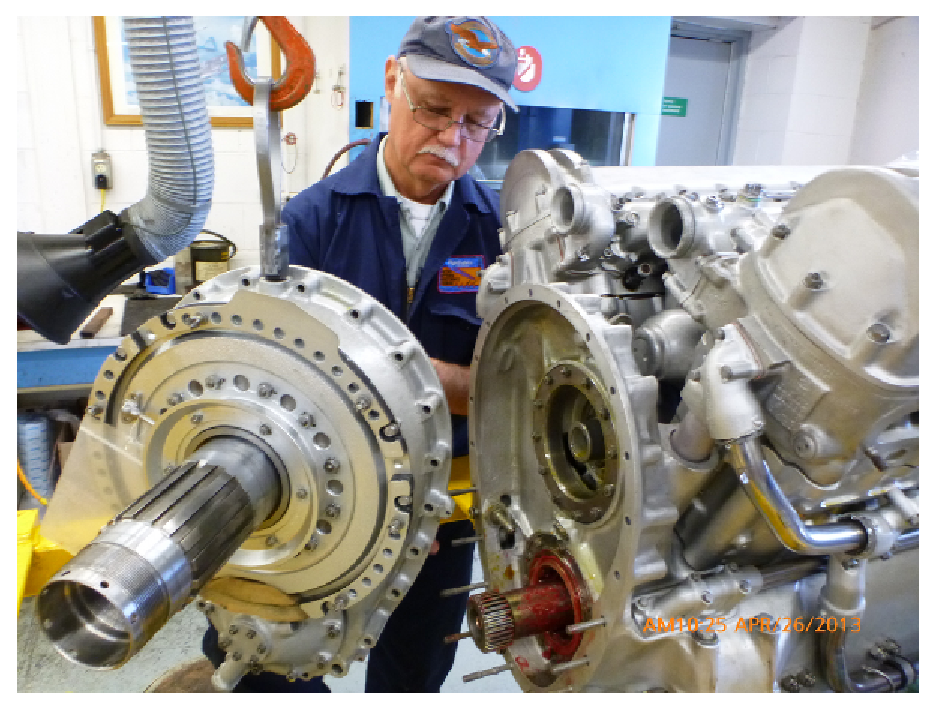
\includegraphics[scale=0.5]{engine3_reduction_gear.eps}
   %caption of the figure 
   \caption*{\small \em Garry Dupont inspecting engine nr 3's
     reduction gearbox.}
   %label of the figure, which has to correspond to \ref{}:
   \label{fig:engine3gearbox}
\end{figure}

Items still requiring restoration are the supercharger and
intercooler, and the auxiliary drive gearbox.  As always, there are
numerous pipes and hoses and fittings that also need attention.  The
engine should be completed by the end of this year.

\section{Engine Frame}
\label{engineframe}

The engine frame was completely disassembled, stripped of paint and
oil, and then repainted and the main components reassembled on the QEC
stand.  The three radiators (water, oil, and intercooler) were
thoroughly cleaned and then repainted and installed.  The cowl support
frame is currently being worked on, but some parts have been added to
the engine frame, along with the fire detectors and fire suppression
system pipes.  The large chin cowl and some of the lower cowls have
been restored.  The top and side cowls still require extensive
restoration.  This work is somewhat hampered by the small number of
volunteers available to work on these items.

\begin{figure}[htbp]
   \vspace{2em}
   \centering
   %name of the graphic, without the path AND in EPS format:
   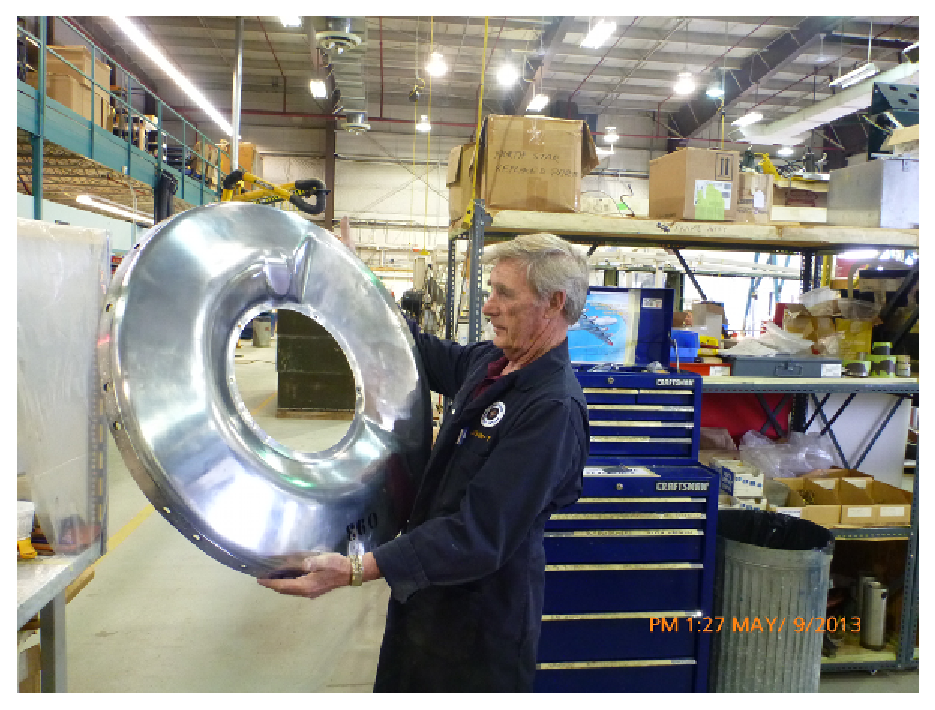
\includegraphics[scale=0.5]{engine3_prop_cowl.eps}
   %caption of the figure 
   \caption*{\small \em John Thibert with the propeller cowl for
     engine nr 3.}
   %label of the figure, which has to correspond to \ref{}:
   \label{fig:engine3propcowl}
\end{figure}


\section{Crew Lounge, Galley,  and Forward Washroom}
\label{crewlounge}

Last spring we removed the equipment from the crew lounge, galley and
forward washroom.  While the aircraft was outside these areas were
cleaned, stripped of paint, then repainted.  The flooring was removed
so the underfloor could be cleaned and primed.  There is some
corrosion damage that must be repaired before new flooring can be
installed.  Most items removed from these areas were restored over the
winter.  This included the washroom door, toilet and washroom
fittings, vanity sink and mirror, and the power inverter installed
opposite the forward washroom.  The old galley was removed and
inspected.  Due to heavy corrosion it was decided to build a
completely new galley, using the old one as a template.  Only the
original doors were retained.  The new galley is complete and will be
stored until it can be installed in the crew lounge.

The heaters had been removed from the ceiling in 2006 and fully
restored, but the air ducts, fuel lines and intake and exhaust scoops
required extensive restoration.  The air scoop was removed from the
aircraft, repaired and re-installed.  The ducts were cleaned, repaired
and new protective heat covers sewn over the old covering.  The water
tank and fittings were removed, cleaned and a new cover sewn over the
tank before installation.  New insulation was installed in the
ceiling, then most heating ducts, cables and pipes were installed.
Several fuel lines had been cut to allow removal of the Janitrol
heaters, and these need to be replaced before the heaters can be
installed.  The doors on the main electrical panel were restored and
installed.  New legends were produced to indicate the circuit breaker
and junction box connections.  These will be laminated and installed
shortly.

\section{Fuselage and Empennage}
\label{empenage}

The rear baggage compartment was cleaned and repainted.  Several floor
panels had stretched and cracked, so new panels were fabricated.  All
panels were stencilled with their respective part numbers before being
installed.  The belly compartment hatch was removed, repaired, painted
and installed.  Recently, the two battery elevators were removed, the
compartment painted, and the elevators will be repainted and installed
shortly.  Batteries were removed when the aircraft arrived at the
museum.  There has been some discussion about obtaining new
(non-functional) batteries to complete this item or work.

Most of the main fuselage was polished while inside the storage
hangar.  The underside and wings still require a lot of work.

Work is progressing on fabricating a complete set of troop seats to
fit up the interior of the main cabin, once this is restored.

\section{Planned Restoration Work--2013}
\label{sec:plannedwork}

Over the next year, we hope to have engine Nr 3 completed and engine
Nr 4 removed.  We will complete the reassembly of the crew lounge and
galley.  We then plan to work on the main cargo compartment, including
refurbishing the main heater duct and other fittings, and removing
floors to begin cleaning and repairs under the cargo floor.  We may
yet get to work on the four engine nacelles.

\section{Membership Report 2012--2013}
\label{sec:membership}

In 2012 we recorded 100 paid members and provided lifetime memberships
to two long serving volunteers and PNSAC Directors, Tim Timmins and
Jim Riddoch.

So far in 2013, we have a total of 66 new or renewed memberships.
This is slightly lower than the same time last year.  Normally, we
would expect to receive a large number of new memberships during
outside displays in the summer, but because of programming changes at
the Museum, our ability to attract new members will be greatly
reduced.

\begin{footnotesize}
  \raggedleft PNSAC\\
\end{footnotesize}

% End of text.

%%% Local Variables: 
%%% mode: latex
%%% TeX-master: main_document.tex
%%% End: 

